\section{Methodology}\label{Methods}
In \hyperref[mcmc used]{\textcolor{blue}{Section }\ref{mcmc used}} the MCMC samplers used in this study are explained in detail. The diagnostics used to evaluate the performance of these samplers are described in \hyperref[mcmc eval]{\textcolor{blue}{Section }\ref{mcmc eval}}. Finally, in \hyperref[mcmc exp]{\textcolor{blue}{Section }\ref{mcmc exp}} the synthetic case studies designed for this study are presented, including the prior and likelihood choices. Everything is implemented in the Python programming language.

\subsection{MCMC samplers used}\label{mcmc used}
Although the simplicity of the Metropolis algorithm is appealing, it is relatively inefficient at exploring the posterior. The algorithms compared in this study attempt to increase this efficiency by utilising different methods to generate proposals for a Markov chain. Opposed to the Metropolis algorithm, these Ensemble Samplers have dependent chains; proposals are generated based on the location of other chains in the ensemble. 

The first MCMC algorithm used in this study is Differential Evolution (DE). \cite{terbraak2006markov} combined the genetic algorithm Differential Evolution \citep{storn1997differential} with MCMC (\hyperref[fig2]{\textcolor{blue}{Figure }\ref{fig2}}). The Differential Evolution algorithm is known in hydrology for it being the main building block of DREAM, the most widely used MCMC method in hydrology. %DE-MC solves an important practical problem in random walk Metropolis, namely that of choosing an appropriate scale and orientation for the jumping distribution

\begin{figure}[ht]
\centering
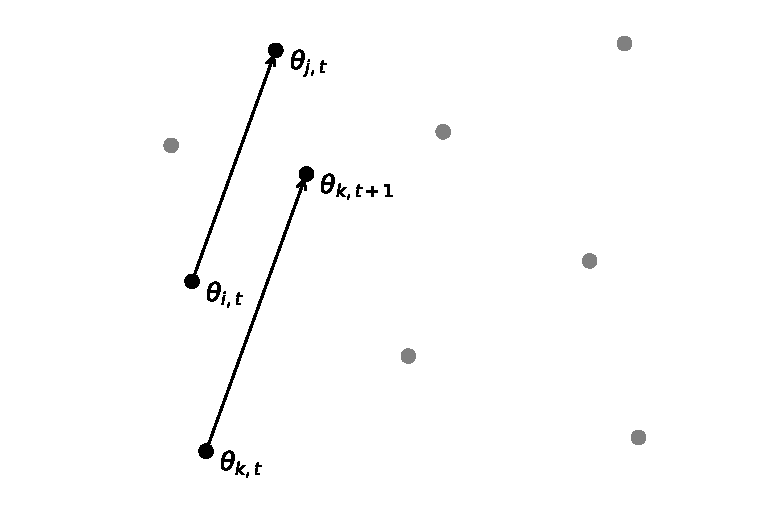
\includegraphics[width=1.0\linewidth]{Figures/DE_move_2025.eps}
\caption{Differential Evolution move for parameter $\theta$ of chain $k$. The grey dots represent the chains not participating. A proposal is generated by randomly selecting two other chains ($i$ and $j$) and superimposing the difference vector of these two chains to the current chain. The difference vector is multiplied by a user-defined scalar (here 1.2), resulting in the proposal $\theta_{k,t+1}$.}\label{fig2}
\end{figure}

The second MCMC algorithm used in this study is Differential Evolution extended with a snooker updater (DE-SNK). \cite{terbraak2008differential} introduced a move called a snooker update to MCMC (\hyperref[fig2b]{\textcolor{blue}{Figure }\ref{fig2b}}).

\begin{figure}[ht]
\centering
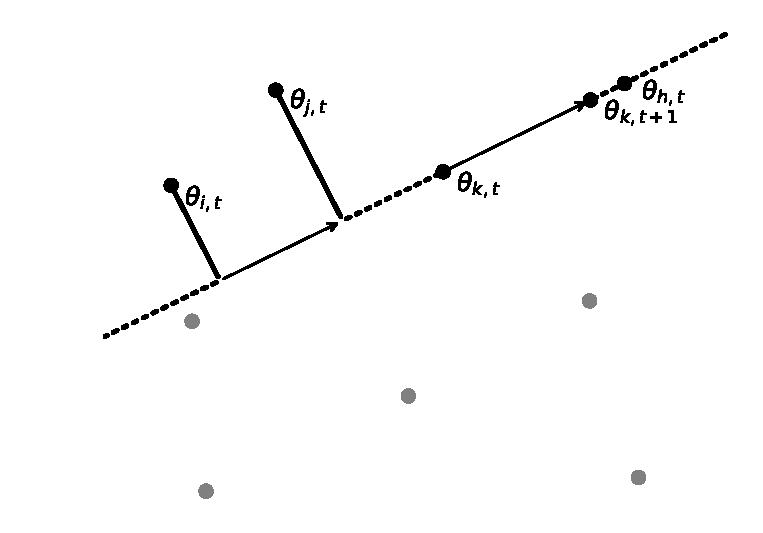
\includegraphics[width=1.0\linewidth]{Figures/snooker_move_2025.eps}
\caption{Snooker update move for chain $k$. A proposal is generated by randomly selecting another chain ($h$) for determining the direction and two chains ($i$ and $j$) for determining the distance. The distance is calculated by projecting $i$ and $j$ orthogonally on the line connecting $k$ to $h$ and subsequently multiplying with a user-defined scalar (here 1.2), resulting in the proposal $\theta_{k,t+1}$.}\label{fig2b}
\end{figure}
\noindent \cite{terbraak2008differential} found that combining Differential Evolution with snooker updates in a 90 to 10 percent ratio leads to the best performance, which is also the setup in this study. They also introduced an algorithm similar to DE-SNK, which requires the use of very few chains (typically 3), by exploiting information from their past by
generating jumps from differences of pairs of past states. Although powerful, sampling from past states was not included as it is not supported by the software used in this study. 

The third and final MCMC algorithm used in this study is the Ensemble Sampler by Goodman and Weare (AI), that utilises the Stretch move (\hyperref[fig1]{\textcolor{blue}{Figure }\ref{fig1}}). \cite{goodman2010ensemble} introduced several affine-invariant MCMC algorithms; hence the name. Here, affine-invariant refers to the algorithm performing well regardless of how skewed the posterior distribution is, e.g. due to strongly correlated parameters. The introduced algorithms utilise different moves, of which the Stretch Move is considered the most powerful \citep{goodman2010ensemble}.

All three samplers are implemented with emcee version 3.1.6 \citep{foreman2013emcee}. Different moves were selected using the \textit{moves} keyword for the (class) \textit{EnsembleSampler}. Since the three samplers only vary in the moves used, selecting different moves results in selecting a different sampler. Optionally, a weighted mixture of moves can be used, as required for DE-SNK. During sampling, at each step, a move is randomly selected from the mixture. For all moves, the default scaling parameters of the emcee package are used, which are consistent with the developers recommendations of said algorithms \citep{terbraak2006markov, terbraak2008differential, goodman2010ensemble}. 

\begin{figure}[ht]
\centering
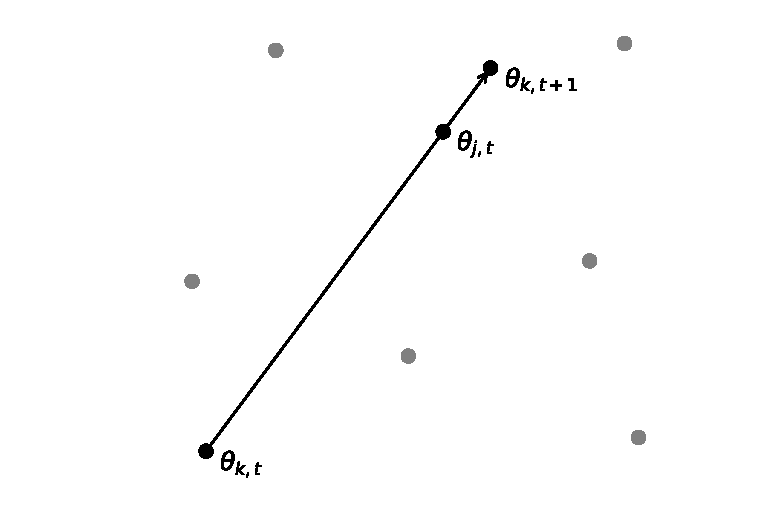
\includegraphics[width=1.0\linewidth]{Figures/stretch_move.eps}
\caption{A stretch move for parameter $\theta$ of chain $k$. The grey dots represent the chains not participating in this move. A proposal is generated by randomly selecting another chain ($j$) and moving in this direction, with the magnitude determined by a user determined scalar (here 1.2), resulting in the proposal $\theta_{k,t+1}$.}\label{fig1}
\end{figure}

\subsection{Performance diagnostics}\label{mcmc eval}
The performance of the different samplers is compared using several diagnostics explained in this section. Chain convergence is evaluated with the Gelman-Rubin diagnostic ($\hat{R}$). Sampling efficiency is assessed with the acceptance rate and the Effective Sample Size (ESS). The posteriors are evaluated on their median, kernel density estimate (KDE) plots and pairs plots. 
%The diagnostics for evaluating the performance of the different samplers are described below. Included are the Integrated Autocorrelation Time, Gelman-Rubin diagnostic, median, acceptance rate, kernel density estimate (KDE) plots and pair plots. % alternatively leave subsection intro empty

\subsubsection{Gelman-Rubin diagnostic}
\cite{gelman1992inference} designed a widely used metric to determine whether one's chains have converged, typically referred to as the Gelman-Rubin diagnostic ($\hat{R}$). This is a ratio between the total variance and the within chain variance (where the total variance is due to both the within and between chain variance).  % can add formulas 13.16 and 13.17 from Students guide to Bayesian statistics.  
As $\hat{R} \to 1$, the chains approach a stationary distribution \citep{lambert2018student}. In practice, when $\hat{R}$ becomes smaller than an arbitrary cutoff value, one's chains are considered to have converged, for which \cite{gelman1992inference} suggested using $\hat{R} \leq 1.1$. 

\cite{gelman2021bayesian} made a small modification to $\hat{R}$, called split-$\hat{R}$, which also compares the first half of each chain to the second half, with the objective to detect lack of convergence within each chain. % \cite{vehtari2021rank} refer to split-R as R, so they consider the 2013 version the new standard...

While very popular, several serious issues have been identified with $\hat{R}$ and split-$\hat{R}$, such as failing to correctly diagnose convergence when the chain has a heavy tail or when the variance varies across the chains. To address these problems, \cite{vehtari2021rank} proposed an alternative rank-based version of $\hat{R}$. In addition \cite{vehtari2021rank} recommends a much more conservative convergence criterion of $\hat{R} \leq 1.01$. 

%Although recommended, 1.01 required impractically long run-times for the hardware used in this study. Therefore, a convergence criterion of 1.05 was used instead. 
The rank-based $\hat{R}$ from \citep{vehtari2021rank} is implemented with the function \textit{rhat} from the \textit{ArviZ} package, version 0.19.0 \citep{kumar2019arviz} and will from now on simply be referred to as $\hat{R}$. 

\subsubsection{Effective Sample Size}
MCMC is a dependent sampling method, resulting in correlation between serial steps of a Markov chain. As a consequence, the effective number of independent samples, called the Effective Sample Size (ESS), is smaller than the total number of steps (\hyperref[eq7a]{\textcolor{blue}{Equation }\ref{eq7a}}).
% definition effective sample size:  how many independent draws contain the same amount of information as the dependent sample obtained by the MCMC algorithm. 
%The correlation between a chain's location and its previous locations is called autocorrelation. The autocorrelation can be computed for different lag values, where lag is the number of steps between the points being compared in the chain. ### This is common knowledge for most hydrologists.
%When the autocorrelation between lagged steps is large and decays slowly, the chain is inefficient and the ESS will be relatively small.

\begin{equation}\label{eq7a}
    \widehat{ESS} = \frac{N}{\hat{\tau}_f}
\end{equation}
Where $N$ represents the total number of steps of the Markov chain and $\hat{\tau}_f$ represents an estimate of the integrated autocorrelation time, which quantifies how many intermediate steps are required for steps to be considered independent. 

For a longer integrated autocorrelation time, more samples must be generated to produce a representative sample of the target density. For a Markov chain $\tau_f$ can theoretically be estimated with \hyperref[eq7]{\textcolor{blue}{Equation} \ref{eq7}}:

\begin{equation}\label{eq7}
    \hat{\tau}_f (N) = 1 + 2 \sum_{\tau=1}^{N} \hat{\rho}_f (\tau) 
\end{equation} 
where $\hat{\tau}_f (N)$ represents an estimate of the integrated autocorrelation time, $N$ represents the number of steps of the Markov chain and $\hat{\rho}_f (\tau)$ represents an estimate of the normalised autocorrelation function. Here, the autocorrelation function is normalised by dividing it by the autocovariance at lag 0.

At larger lags, $\hat{\rho}_f (\tau)$ starts to contain more noise than signal, summing up to N will therefore lead to a noisy estimate of $\hat{\tau}_f$. Instead, \cite{sokal1997monte} recommends estimating $\tau_f$, for some $M \ll N$, with \hyperref[eq8]{\textcolor{blue}{Equation} \ref{eq8}}:  
\begin{equation}\label{eq8}
    \hat{\tau}_f (M) = 1 + 2 \sum_{\tau=1}^{M} \hat{\rho}_f (\tau) 
\end{equation} 
By introducing $M$, the function is evaluated for a smaller number of lags, decreasing the variance at the cost of a small increase in bias.  \cite{sokal1997monte} recommends choosing the smallest value of $M$, where $M \geq C \, \hat{\tau}_f (M)$ and $C \sim 5$. For an extensive discussion on computing the integrated autocorrelation time the reader is referred to %'see' feels informal
\cite{sokal1997monte}, or to \cite{foreman2022autocorr} for a summary of the most important points. %not sure how to cite foreman2022autocorr 
%Sokal says that he finds this procedure to work well for chains longer than, but the situation is a bit better with emcee because we can use the parallel chains to reduce the variance and we’ve found that chains longer than about are often sufficient
Here, $\hat{\tau}_f (M)$ was computed with the function 
\textit{autocorr.integrated\_time}
from the \textit{emcee} package, version 3.1.6 \citep{foreman2013emcee}.

\subsubsection{Other diagnostics}
Generally, groundwater flow models have a constant value for each parameter. On the other hand, MCMC produces an estimated posterior distribution for each parameter. This introduces the challenge of choosing the most suitable value from this distribution to use in the groundwater flow model. Possible options include the distribution mean, median, or mode. The mean has the drawback that it is strongly influenced by extreme values. This is problematic because, the the posterior distributions of the parameters in this study span multiple orders of magnitude. Selecting the mode of the distribution may be an intuitive value to use in the groundwater flow model. However, problems arise when the distribution is multimodal (the tallest mode, may e.g. have little width, making it challenging to select a mode). Since the median does not have the drawbacks of the mean and mode, it has been selected as the point estimator to use for parameters in MODFLOW 6. %In this study the ensemble median has been selected for this purpose. % specify that the median was implemented with scripts developed by the author?

The fraction of proposed steps that are accepted is called the acceptance rate, giving an indication of sampling efficiency. If the acceptance rate approaches 1, most proposals are accepted, resulting in inefficient random-walk behaviour. An acceptance rate close to 0 on the other hand, results in inefficiency due to the chain being mostly stuck in the same place. 

\cite{gelman1997weak} found that optimal acceptance rates for the Metropolis algorithm scale with dimensionality (number of calibrated parameters), starting at about 0.44 for 1 dimension and decreasing to about 0.23 for highly dimensional problems. The optimal acceptance rate decreases with dimensionality because, for higher dimensional problems, the 'volume' containing posterior density becomes increasingly small relative to the remainder of parameter space \citep{mackay2003information}. Although the optimal acceptance rates found by \cite{gelman1997weak} are for the Metropolis algorithm, the results are widely used as a guideline for other samplers, including by \cite{terbraak2006markov} for DE. More recently \cite{schmon2022optimal} found optimal Metropolis acceptance rates for specific dimensional problems. By adjusting the tuning parameters of a sampler (e.g. the width of the proposal distribution for Metropolis), different acceptance rates can be achieved. However, for Ensemble Samplers, default tuning parameters are typically used (also in this study, see \hyperref[mcmc used]{\textcolor{blue}{Section }\ref{mcmc used}}). Therefore, considering sampling efficiency, it is useful to examine whether default tuning parameters for the samplers used in this study result in (close to) optimal acceptance rates. %No existing Python packages were used to compute the acceptance rates, but scripts developed by the author. OR leave it out because by not mentioning I imply that I wrote these scripts?

Kernel density estimate (KDE) plots represent the posterior samples using a continuous probability density curve, providing a clear visualization of the posterior distributions of each parameter. KDE plots were used for identifying multimodality and for comparing the posteriors produced by different samplers. %and scenarios
KDE plots were implemented using the function \textit{kdeplot} from the \textit{Seaborn} package, version 0.13.2 \citep{Waskom2021}.

A pairs plot is a matrix of graphs that visualizes the relationship between parameters by pairwise comparison. It combines both histogram and scatter plots, providing an overview of estimated posterior distributions and parameter covariance. Pairs plots were implemented (with a KDE style) using the function \textit{pairplot} from the \textit{Seaborn} package. % repeat version or not? 

\subsection{Synthetic scenarios}\label{mcmc exp}
The MCMC samplers (DE, DE-SNK and AI) are compared in a calibration exercise. Four simple steady-state synthetic groundwater flow models (designed using MODFLOW 6) were calibrated, which are described in \hyperref[gfm]{\textcolor{blue}{Section }\ref{gfm}}. The performance of the samplers is evaluated in different scenarios, in which not only different models are used, but also different priors and number of observations, as described in \hyperref[mcmc setup]{\textcolor{blue}{Section }\ref{mcmc setup}}.

\subsubsection{Groundwater flow models}\label{gfm}
The four synthetic groundwater flow models designed for this study are shown in \hyperref[fig_sgm]{\textcolor{blue}{Figure }\ref{fig_sgm}}. These models were developed using MODFLOW 6, version 6.5.0 \citep{langevin2017modflow}. To create, run and post-process these models, FloPy version 3.8.1 was used \citep{hughes2023flopy}. The parameters $inner\_maximum$ and $outer\_maximum$ from FloPy's Iterative Model Solution package were both increased from their default values (25 and 50, respectively) to 1000, allowing more iterations for the solver. This solved MODFLOW simulation errors encountered during testing runs (\hyperref[sim_error]{\textcolor{blue}{Appendix }\ref{sim_error}}). 

The hydraulic conductivities presented in \hyperref[fig_sgm]{\textcolor{blue}{Figure }\ref{fig_sgm}} represent the 'true' values for each model. Running each model with these 'true' hydraulic conductivities results in the 'true' hydraulic heads for every model cell. With the well located in the phreatic layer in every model, one would expect flow paths to be towards the well for all layers. This is indeed the case as can be seen by the deeper layers having increasingly large hydraulic heads (\hyperref[fig_heads_side]{\textcolor{blue}{Figure }\ref{fig_heads_side}}).

To simulate the effects of measurement errors of hydraulic head measurements performed in the field, noise was added to the ’true’ hydraulic heads of every model cell. \cite{rau2019error} compared eight different electric dip meters and found that the random measurement error varied by several centimeters depending on the operator and the water depth. Furthermore, it was

\begin{figure}[ht]
\centering
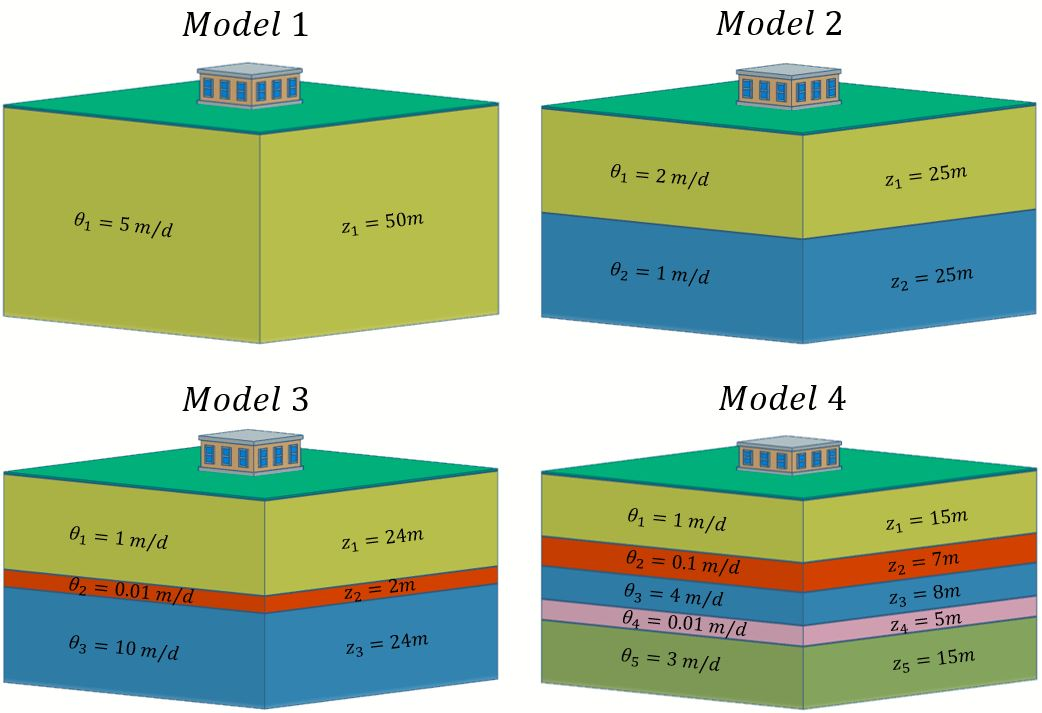
\includegraphics[width=1.0\linewidth]{Figures/CONGROMO_NEW4.JPG}
\caption{Schematic of the four steady-state synthetic groundwater flow models used in this study. Layer thickness ($z_n$) and the respective isotropic hydraulic conductivities ($\theta_n$) are shown inside each layer ($n$). The models have a length and width of 1000 meters, consisting of 25 rows and columns with a length of 40 meters. The total depth of each model equals 50 meters. At the centre of each model is an abstraction well (indicated by the building) with an extraction rate of 500 m\textsuperscript{3}/day. The well screens extend over the full depth of the phreatic aquifer of the respective model, resulting in e.g. a 50 meter long well screen for Model 1, versus a 15 meter long well screen for Model 4. At the model edges, there are constant head boundaries of 10 meters.}\label{fig_sgm} %so the location of the label influences how it is referenced!?, that's clunky
\end{figure} %Above each model, its name is given with the number of calibrated parameters indicated by the subscript.

\begin{figure}[htb!]
\centering
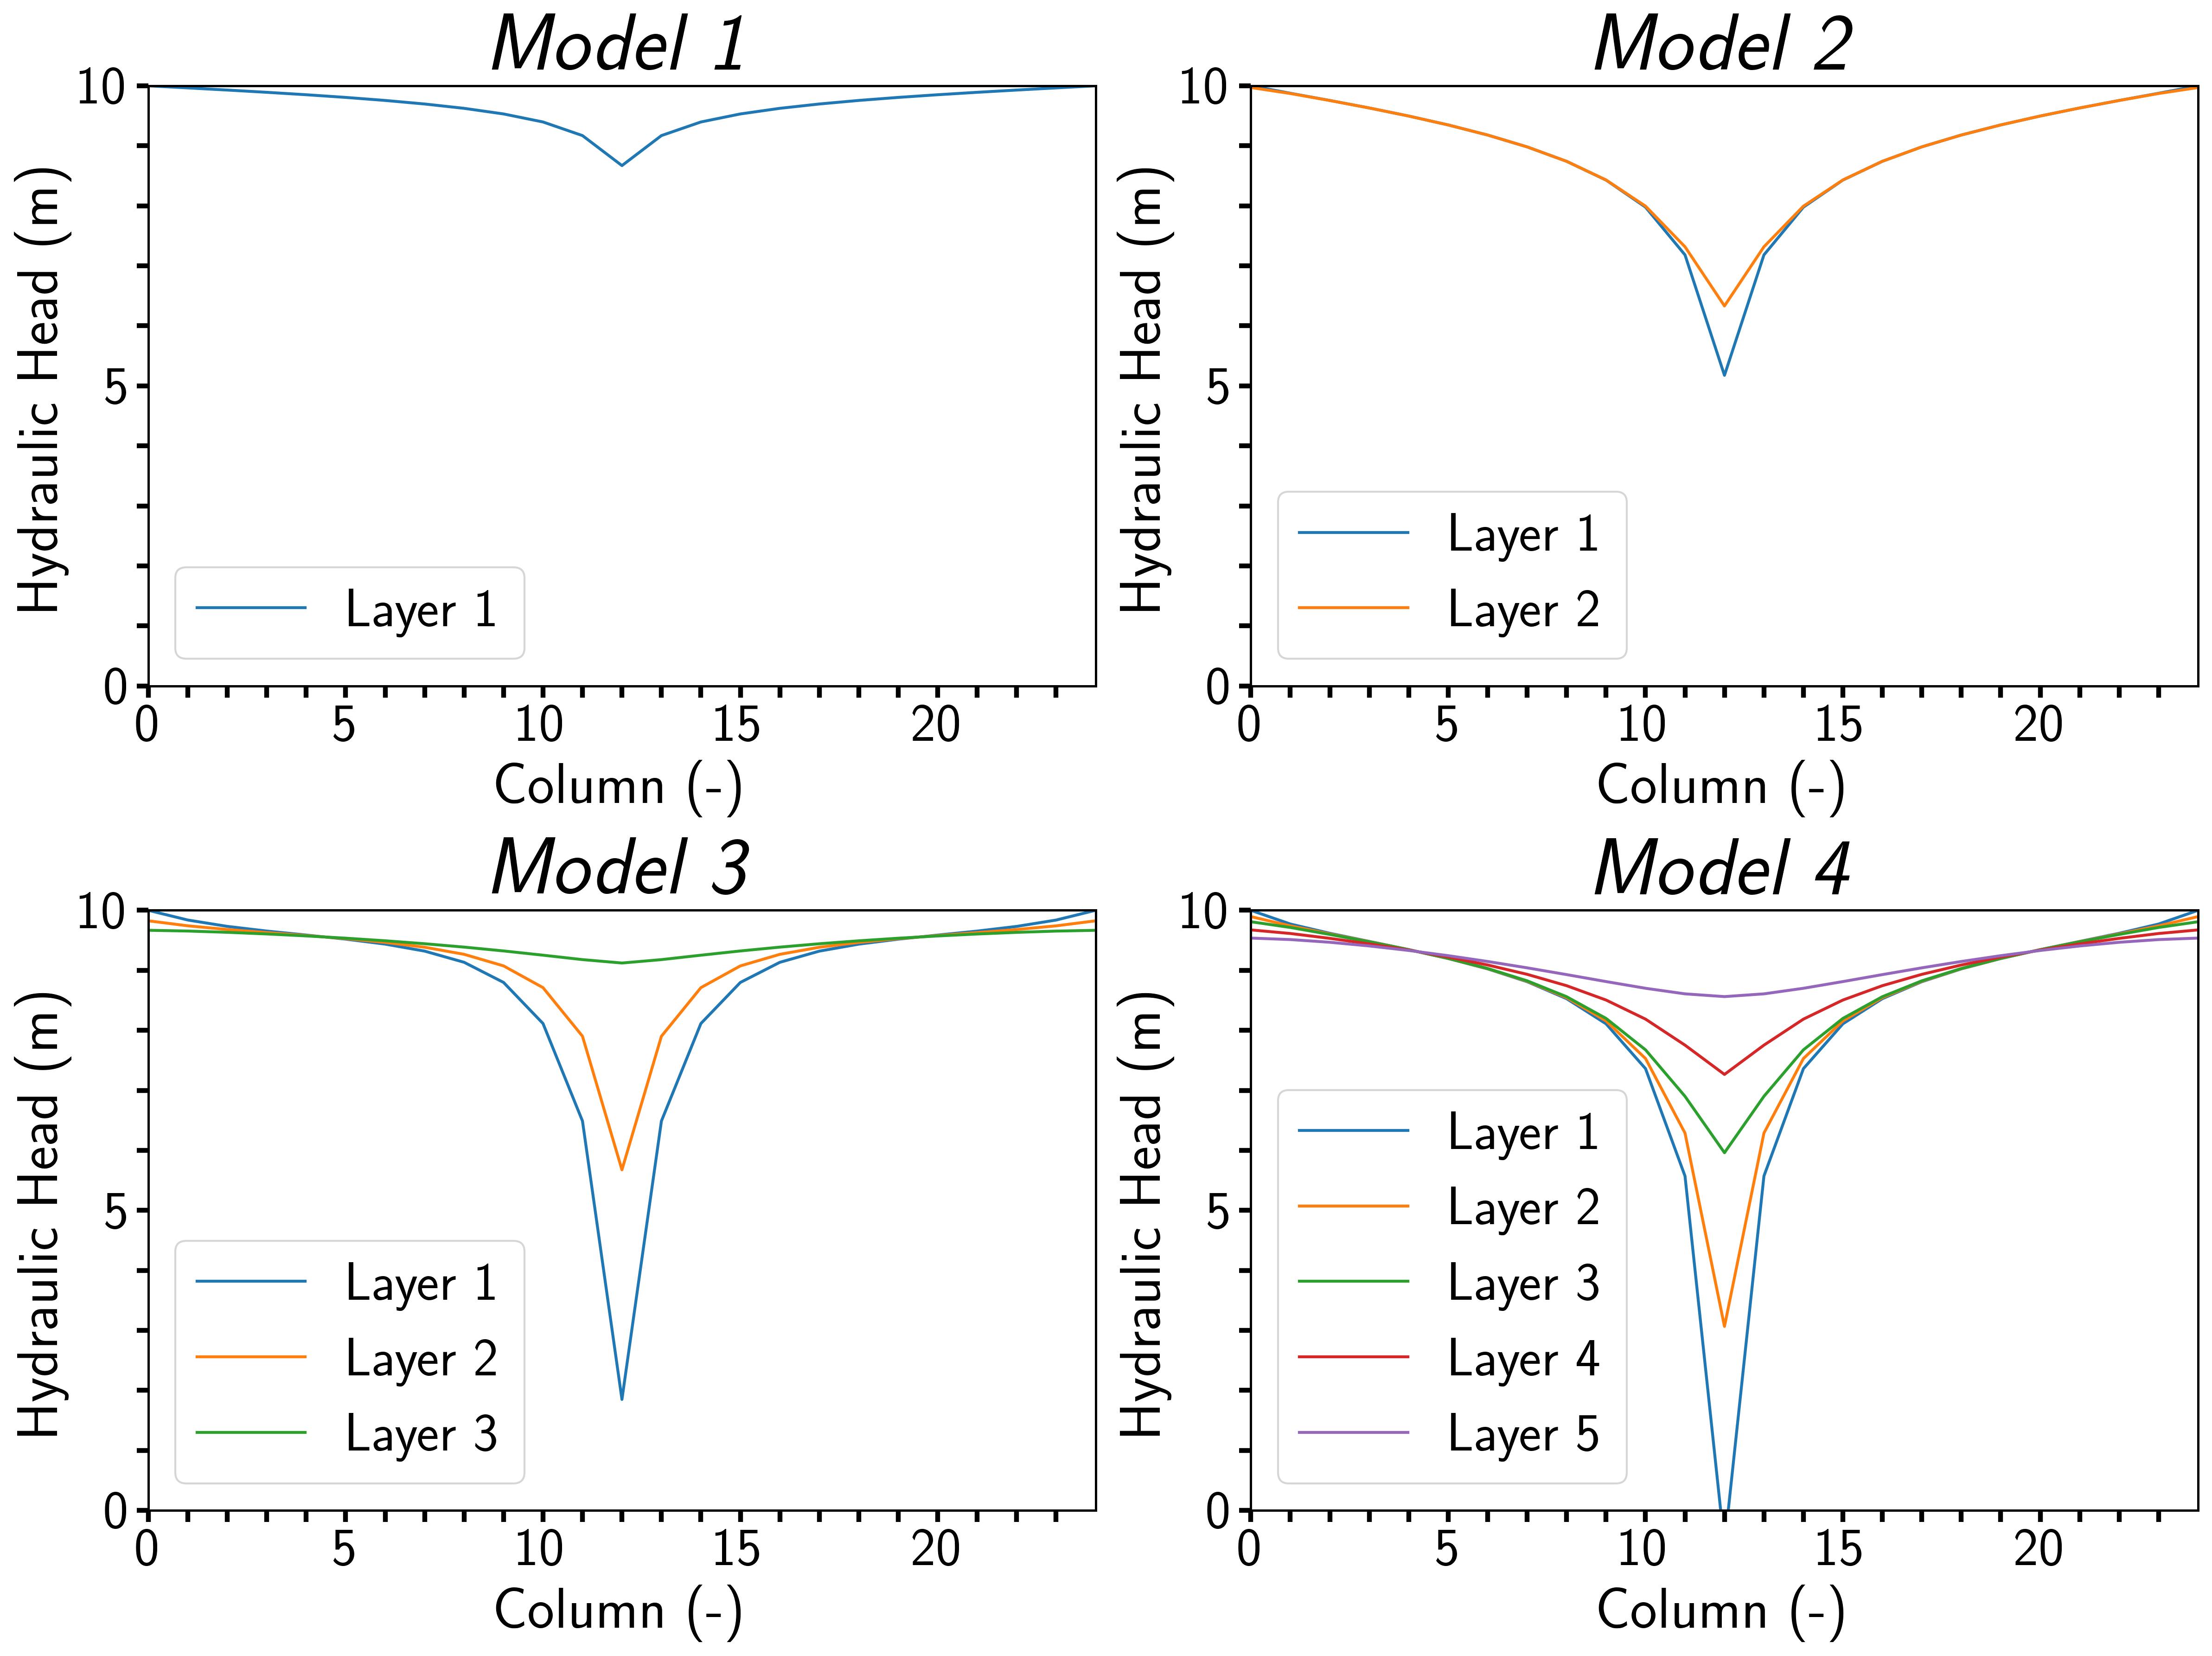
\includegraphics[width=1.0\linewidth]{Figures/heads_side.png}
\caption{Side view of the true hydraulic heads (m) in all models. The side view shows row 12 out of 25 rows total, indexing from 0. The x axis shows the columns of the different models (also 25 total). Note that layer 1 always refers to the uppermost layer, with deeper layers having sequentially greater numbers.\label{fig_heads_side}}
\end{figure} % fix widt back to 1 possibly as it looks nicer

\noindent shown by \cite{rau2019error} that the magnitude of systematic errors tends to be much larger than that 

\begin{table*}[htb]
\caption{Priors for the hydraulic conductivities in the designed groundwater flow models. The presented prior distributions (truncated normal) are transformed for use by the MCMC samplers\textsuperscript{[1]}. For each prior, a formula is presented to transform the respective parameter as used in MCMC ($\theta_{\text{mc}}$), to a hydraulic conductivity in m/d ($\theta_{\text{mod}}$). For the narrow prior, $\mathcal{O}$ is introduced, which represents log10() of the 'true' hydraulic conductivity (m/d), subsequently rounded down to an integer (in python: math.floor(math.log10(x))).}
\label{tab_priors}
\setlength{\tabcolsep}{13pt} %can manually adjust column spacing
\begin{tabularx}{\textwidth}{lllll}
\toprule
Name & Sediment & Prior distribution & Transformation (m/d) & bounds (m/d) \\
\midrule
Wide & clean sand & $\mathcal{TN}(0, 0.5^2, -1, 1)$ & $\theta_{\text{mod}} = 10^{2\theta_{\text{mc}} + 1}$ & [$10^{-1},10^3]$\\
Wide & silty sand  & $\mathcal{TN}(0, 0.5^2, -1, 1)$ & $\theta_{\text{mod}} = 10^{2\theta_{\text{mc}}}$ &  [$10^{-2},10^2]$\\
Wide & silt, loess   & $\mathcal{TN}(0, 0.5^2, -1, 1)$  & $\theta_{\text{mod}} = 10^{2\theta_{\text{mc}} - 1}$  & [$10^{-3},10^1]$\\
\midrule
Narrow & - & $\mathcal{TN}(0, 0.125^2, -1, 1)$  &  $\theta_{\text{mod}} = 10^{2\theta_{\text{mc}} + \mathcal{O}}$ & [$10^{-2+\mathcal{O}},10^{2+\mathcal{O}}]$\\
\bottomrule
\end{tabularx}
\end{table*}

\noindent of random errors. Systematic errors can have a constant bias (e.g. poorly calibrated equipment) or a non-constant bias (e.g. salinity can result in a linearly increasing bias with depth due to density differences compared to fresh water). %, similarly a borehole drilled under an angle can result in linearly increasing bias with depth). 
For simplicity, all errors were lumped into a Gaussian distribution with an inflated variance based on these findings. Measurement noise was added $\epsilon \sim N(0,0.1)$, with the mean and standard deviation in meters.

After adding noise to all hydraulic heads, observation locations were selected stochastically. This was achieved by randomly generating numbers between 2 and 24 using the function \textit{randint} from Python's built-in \textit{random} module, with each number specifying the row or column of a cell in the model. Cells on the boundary of the model, with corresponding row and column integers of 1 and 25, are excluded from being selected as measurement locations, due to the boundary conditions at the edges of the models. If by chance the same x,y coordinates are selected more than once, resampling occurs. If the model has multiple layers, selected observations are always on top of each other, similar to how one measurement well contains multiple piezometers in different layers. 

To provide insight into the importance of the amount of available data, three scenarios per model were created. The scenarios differ in the number of observations per layer: 1, 3 or 5. For a more complex model this results in a greater number of total observations than a simpler model, but in the same amount of observations per layer (i.e. per parameter). 

\subsubsection{MCMC setup}\label{mcmc setup}
Six different prior-likelihood combinations (scenarios) were created for each of the four synthetic groundwater flow models shown in \hyperref[fig_sgm]{\textcolor{blue}{Figure }\ref{fig_sgm}}. These scenarios differ in: prior knowledge (on hydraulic conductivities) and available data (number of hydraulic head measurements for computing the likelihood). 

The priors are similar to what may be used in a real case study, by using representative values of the respective sediments/geological materials. For each layer of each model two different priors were created, from now on referred to as the narrow and wide prior. 

The wide priors are based on lithology (supposedly) found in the respective layers during e.g. piezometer construction. The prior bounds for hydraulic conductivities are inspired by the ranges for clean sand, silty sand, and silt presented in \cite{woessner2020hydrogeologic}. The 'true' hydraulic conductivity value of each layer was designed to fall within the prior bounds of the lithology found within each layer (see \hyperref[tab_priors]{\textcolor{blue}{Table }\ref{tab_priors}} for the priors and \hyperref[tab_priors_lithology]{\textcolor{blue}{Appendix }\ref{tab_priors_lithology}} for the lithology of each layer). 

\begin{figure}[htb]
\centering
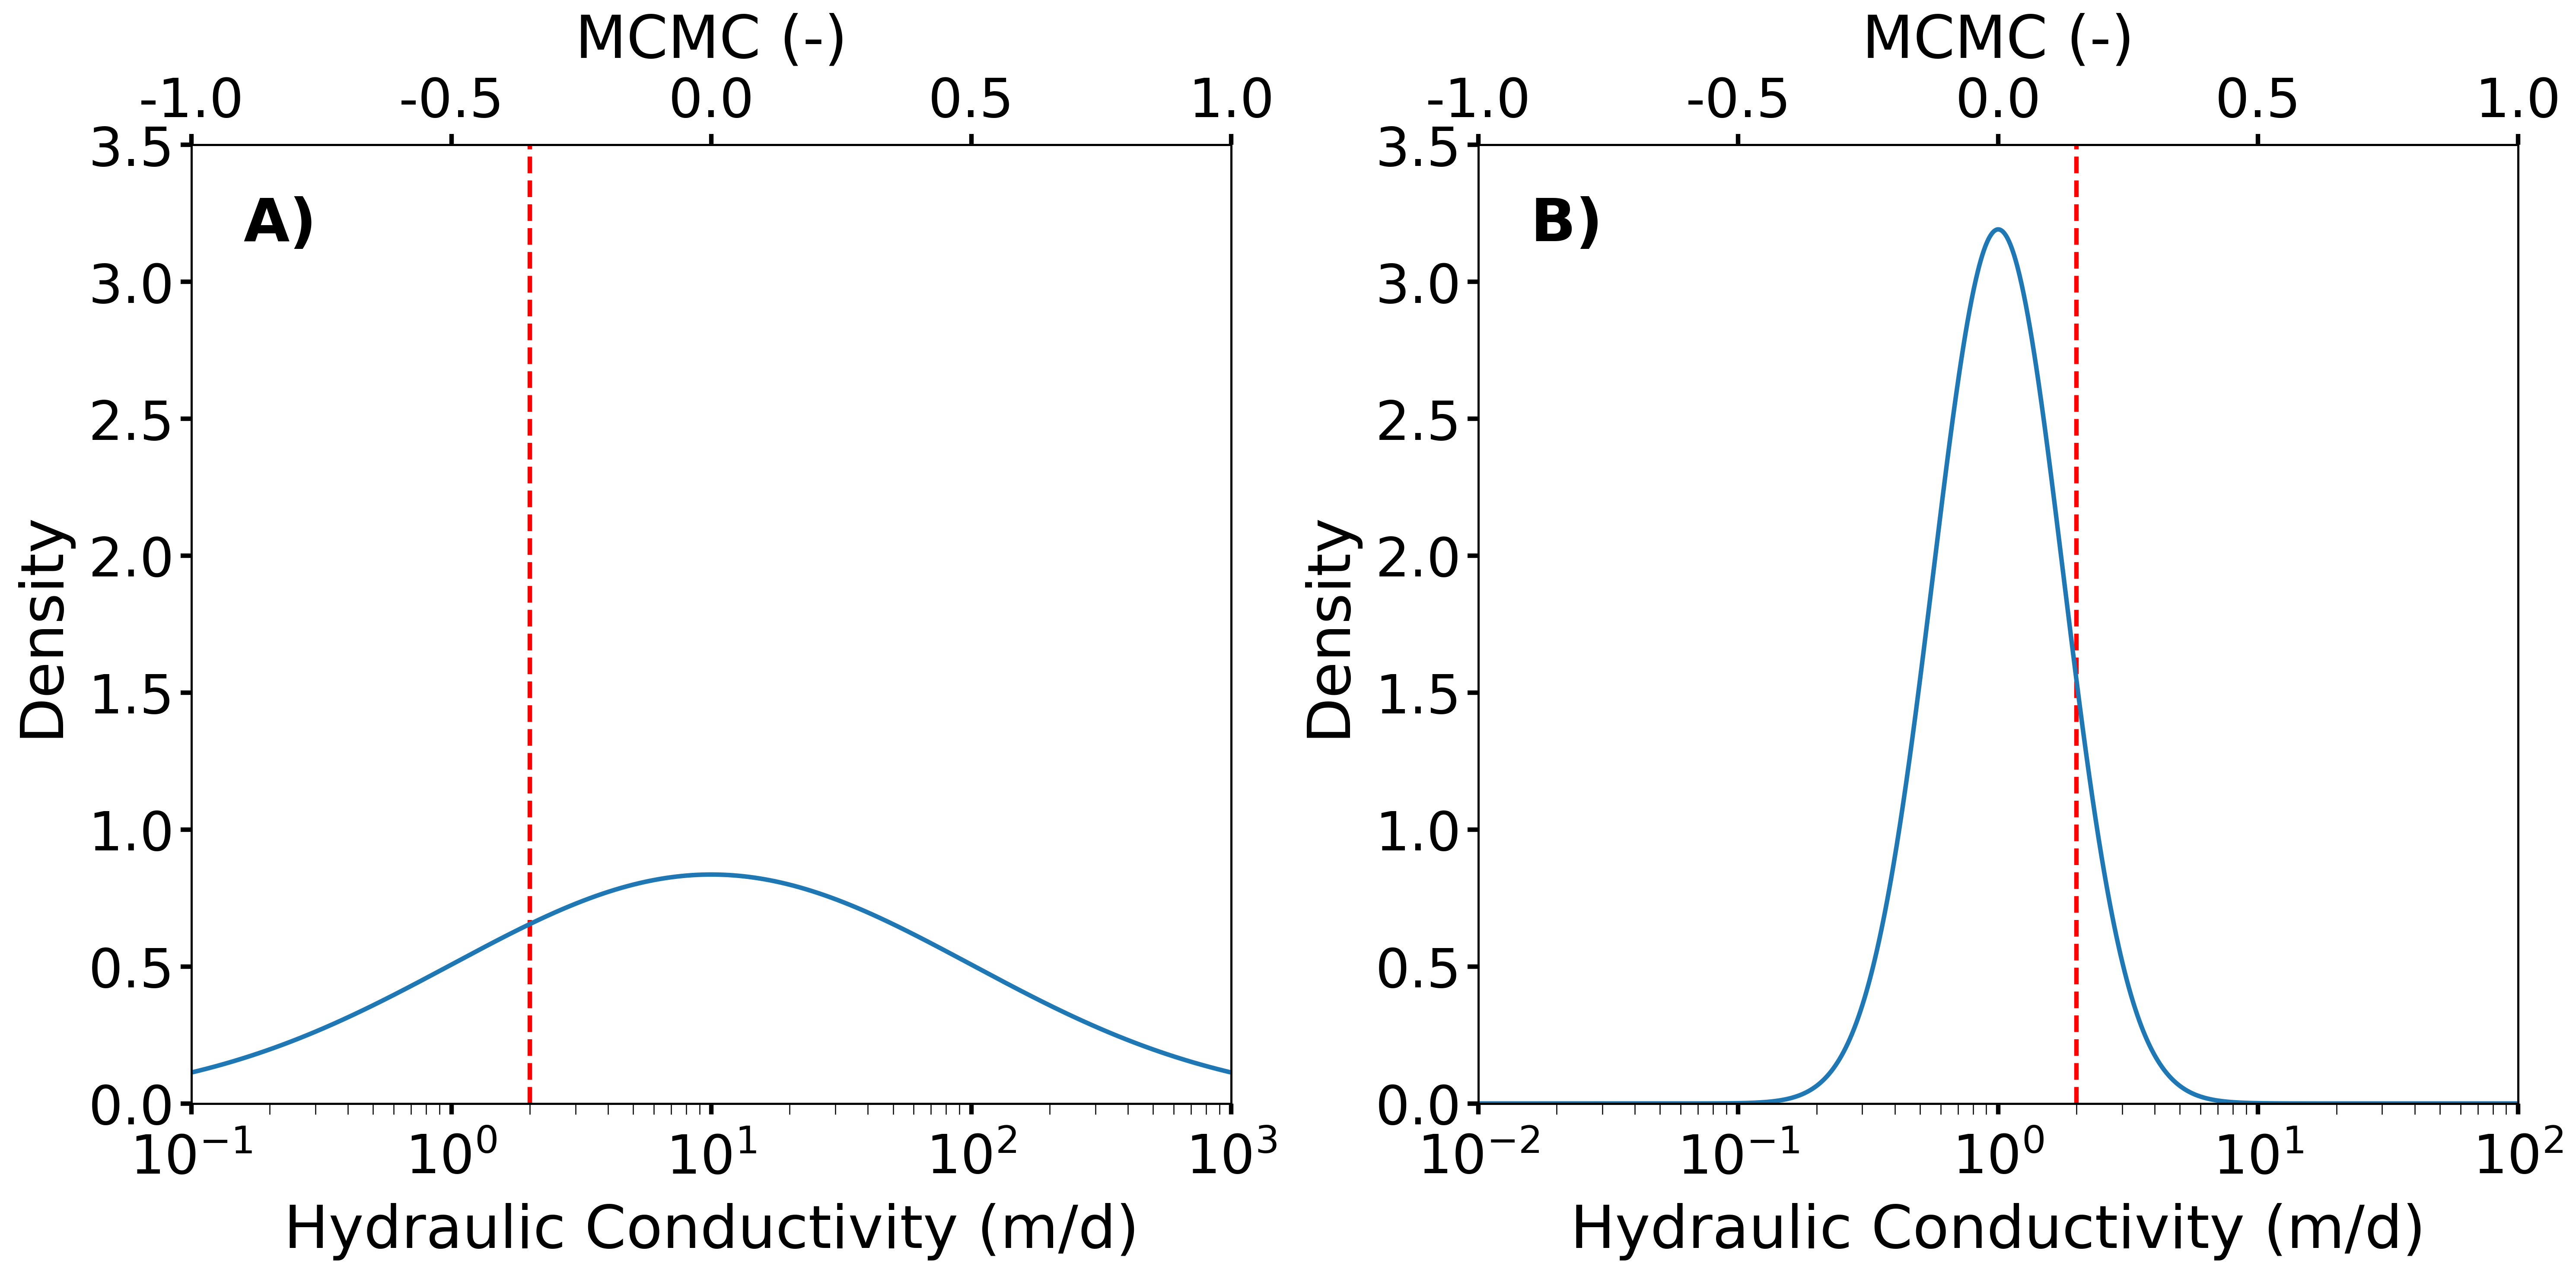
\includegraphics[width=1.0\linewidth]{Figures/priors.png}
\caption{Prior distributions for the hydraulic conductivity of layer 1 in Model 2 (contains clean sand), with \textbf{A)} showing the wide prior and \textbf{B)} the narrow prior. The top x-axes indicate the parameter values used by the MCMC algorithm, while the bottom x-axes show the corresponding transformed hydraulic conductivity values (m/d) as used by MODFLOW 6. The priors are truncated at the plot boundaries. The dotted red line indicates the true hydraulic conductivity.}\label{fig_priors}
\end{figure} 

\footnotetext[1]{The applied parameter transformations differ from statistical convention. Conventionally, the transformation for the likelihood function would simply take the exponent of the parameter: $\theta_{mod} = 10^{\theta_{mc}}$. The prior for e.g. clean sand would then be $\mathcal{TN}(1, 1, -1, 3)$ and the prior for silty sand would be $\mathcal{TN}(0, 1, -2, 2)$. However, the result of both methods on inference is the same.}% can replace methods with approaches

For the narrow prior, it is assumed that a much more precise estimate of the hydraulic conductivity of each layer is available (e.g. from pumping tests). The narrow priors have a standard deviation four times smaller than that of the wide priors. Additionally, the centre of the narrow prior distribution depends on the 'true' hydraulic conductivity (\hyperref[tab_priors]{\textcolor{blue}{Table }\ref{tab_priors}}). Note that the centre of the narrow prior is within an order of magnitude distance from the 'true' hydraulic conductivity (\hyperref[tab_priors]{\textcolor{blue}{Table }\ref{tab_priors}}). An example of the narrow and wide prior distributions is shown in \hyperref[fig_priors]{\textcolor{blue}{Figure }\ref{fig_priors}}. 

With hydraulic conductivities spanning many orders of magnitude, numerical stability of the MCMC samplers was a concern. Parameter transformation was applied to address this issue. The parameters were transformed at each step of the Markov chain, to a hydraulic conductivity in meters per day (\hyperref[tab_priors]{\textcolor{blue}{Table }\ref{tab_priors}}). 
Subsequently, the respective model was run in MODFLOW 6 with the transformed parameters. For each selected observation location, the difference was calculated between the hydraulic heads produced by this model run and the noisy observations ($\delta h$). For each observation, $\delta h$ was inserted into the log probability density function (logpdf) of the error. The log-likelihood was computed as the sum of the logpdf of every observation. The selected likelihood distribution is $\mathcal{N}(0,0.1)$, which is identical to the distribution that was used to generate the measurement noise. % is this a correct likelihood?
Priors and likelihood were implemented with the functions \textit{truncnorm}, \textit{norm} and \textit{logpdf} from the \textit{SciPy.stats} package, version 1.11.4 \citep{2020SciPy-NMeth}. % or module?
% no Jacobian adjustment was necesarry because: the difference between a change of variables and a simple variable transformation. A transformation samples a parameter, then transforms it, whereas a change of variables transforms a parameter, then samples it. Only the latter requires a Jacobian adjustment. https://mc-stan.org/docs/stan-users-guide/reparameterization.html#changes-of-variables

Chain initialisation was performed by taking a random sample from the respective prior distribution with the \textit{rvs} function from the \textit{SciPy.stats} package. This was programmed with a constant seed, to ensure that identical datasets were used for chain initialisation of different samplers and scenarios.

For each of the six scenarios (prior-likelihood combinations), five ensembles were run per sampler (AI, DE and DE-SNK), each consisting of 10 chains with a length of 2000 steps. This procedure was carried out for all (four) designed synthetic groundwater flow models. Trace plots of testing runs showed good mixing of the Markov chains within 1000 steps. Therefore, burn-in was set at 1000 steps, leaving 1000 steps per chain for estimation of the posterior distribution. 

\newpage